\subsubsection{Dịch vụ nhân vật (persona service)}

% Mục đích:
Chịu trách nhiệm quản lý hệ thống nhân vật (personas), kho giọng đọc (\texttt{Voices}), các nền tảng tổng hợp giọng nói (\texttt{TTS Engines}) và xử lý trực tiếp các yêu cầu chuyển đổi văn bản thành âm thanh (\texttt{Text-to-Speech}).

\begin{figure}[H]
\centering
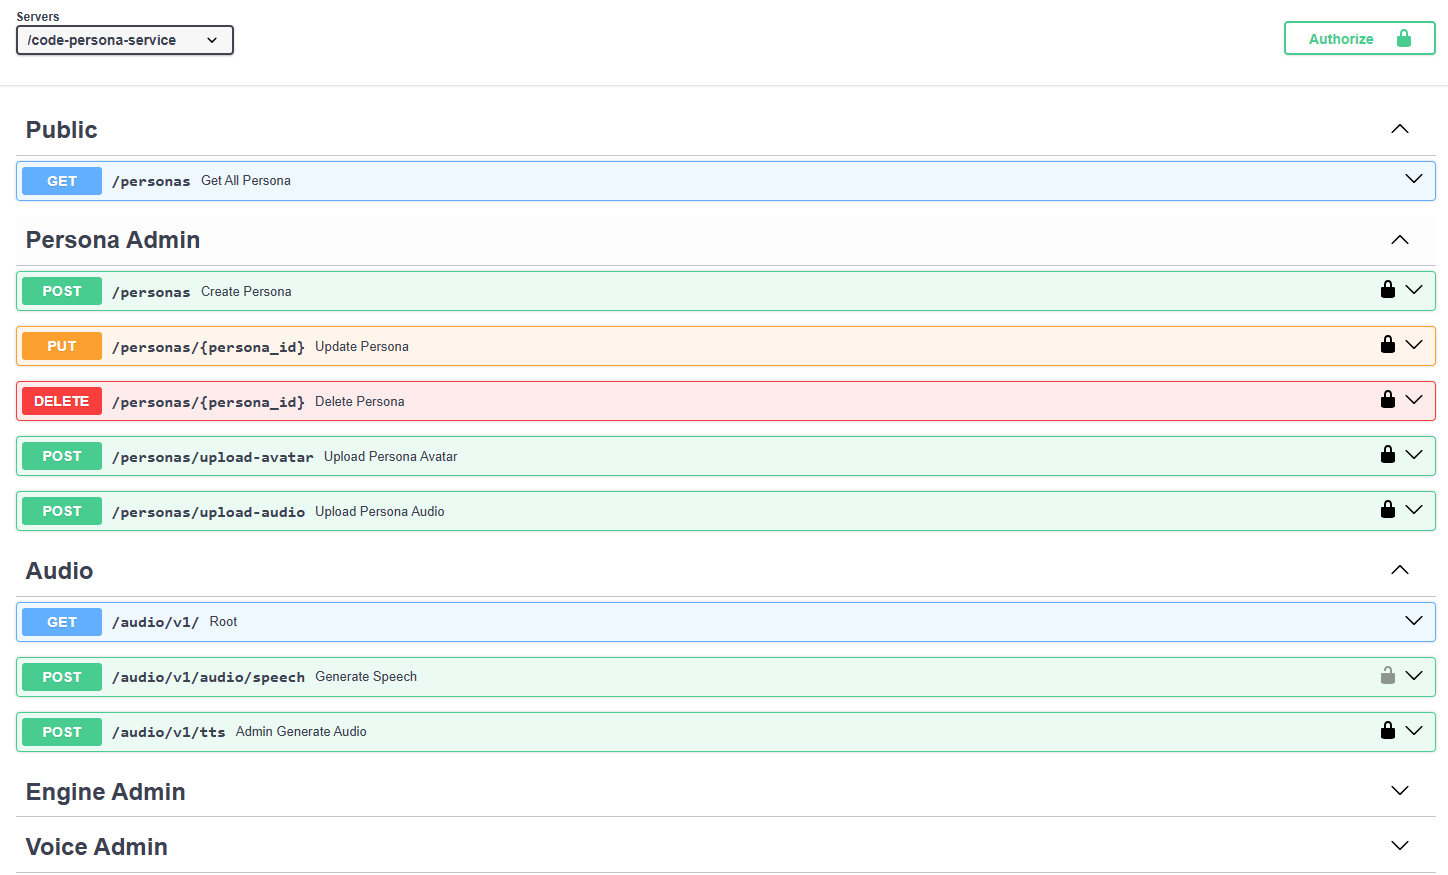
\includegraphics[width=0.95\textwidth]{pictures/persona-swagger2.png}
\caption{Tài liệu Swagger API dịch vụ nhân vật}
\end{figure}

\paragraph{Các chức năng chính}

\begin{itemize}
\item \textbf{Truy xuất danh sách nhân vật}: Cung cấp danh sách các nhân vật trong hệ thống, hỗ trợ phân trang và lọc theo \texttt{persona\_id}.

\item \textbf{Quản lý nhân vật (Dành cho ADMIN)}: Cho phép tạo mới, cập nhật thông tin hoặc xóa bỏ các nhân vật khỏi hệ thống. Tải lên hình ảnh đại diện (\texttt{avatar}) và file âm thanh câu chào mẫu (welcome audio) cho từng nhân vật.

\item \textbf{Quản lý công cụ TTS (engines)}: Cho phép quản trị viên ADMIN định nghĩa, cập nhật, xóa và truy xuất danh sách các nền tảng dịch vụ cung cấp TTS.

\item \textbf{Quản lý giọng đọc (voices)}: Cho phép tạo, cập nhật, xóa và truy xuất danh sách các giọng đọc cụ thể, hỗ trợ bộ lọc theo công cụ/nền tảng.

\item \textbf{Đồng bộ ElevenLabs}: Tích hợp API đồng bộ danh sách giọng đọc mới nhất từ nhà cung cấp ElevenLabs trực tiếp về hệ thống CSDL.

\item \textbf{Chuyển đổi Text-to-Speech}: Cung cấp chức năng tạo ra âm thanh từ văn bản đầu vào thông qua hai thư viện: \texttt{edge-tts} (tổng hợp online) và \texttt{piper-tts} (tổng hợp offline chất lượng cao). Với \texttt{piper-tts}, hệ thống yêu cầu tệp mô hình giọng đọc được lưu trữ tại Cloudflare R2 và tự động tải xuống máy chủ cục bộ khi dịch vụ bắt đầu khởi động.

\item \textbf{Cơ chế Cache tối ưu (TTS Caching)}: Sử dụng \textbf{Disk Cache} (thư viện \texttt{diskcache} cơ chế LRU, kích thước giới hạn 1GB) để lưu giữ các file âm thanh đã tổng hợp lên ổ đĩa nhằm phản hồi tức thì các yêu cầu trùng lặp và sử dụng \textbf{Memory Cache} để lưu giữ các đối tượng mô hình Piper đã load vào bộ nhớ RAM (\texttt{\_loaded\_voices}), tránh việc phải nạp lại tệp tin mô hình \texttt{.onnx} nặng sau mỗi yêu cầu, tối ưu tốc độ phát âm thanh.

\item \textbf{Lưu trữ tài nguyên}: Toàn bộ dữ liệu mẫu âm thanh (\texttt{audio}), hình ảnh (\texttt{images}) và mô hình (\texttt{models}) phục vụ cho dịch vụ nhân vật được lưu trữ an toàn tại Cloudflare R2.
\end{itemize}

Quản lý thư mục tài nguyên của dịch vụ nhân vật trên Cloudflare R2:

\begin{figure}[H]
\centering
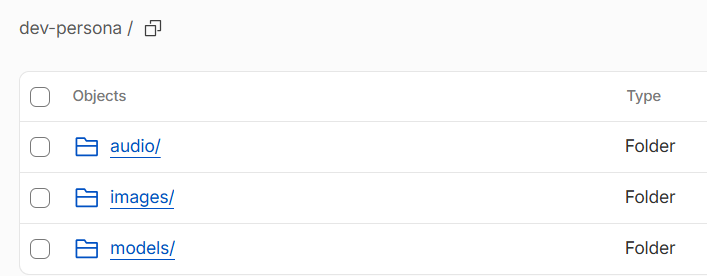
\includegraphics[width=0.8\textwidth]{pictures/r2per.png}
\caption{Tài nguyên nhân vật lưu trữ trên Cloudflare R2}
\end{figure}

Quản lý di chuyển CSDL của dịch vụ nhân vật:

\begin{figure}[H]
\centering
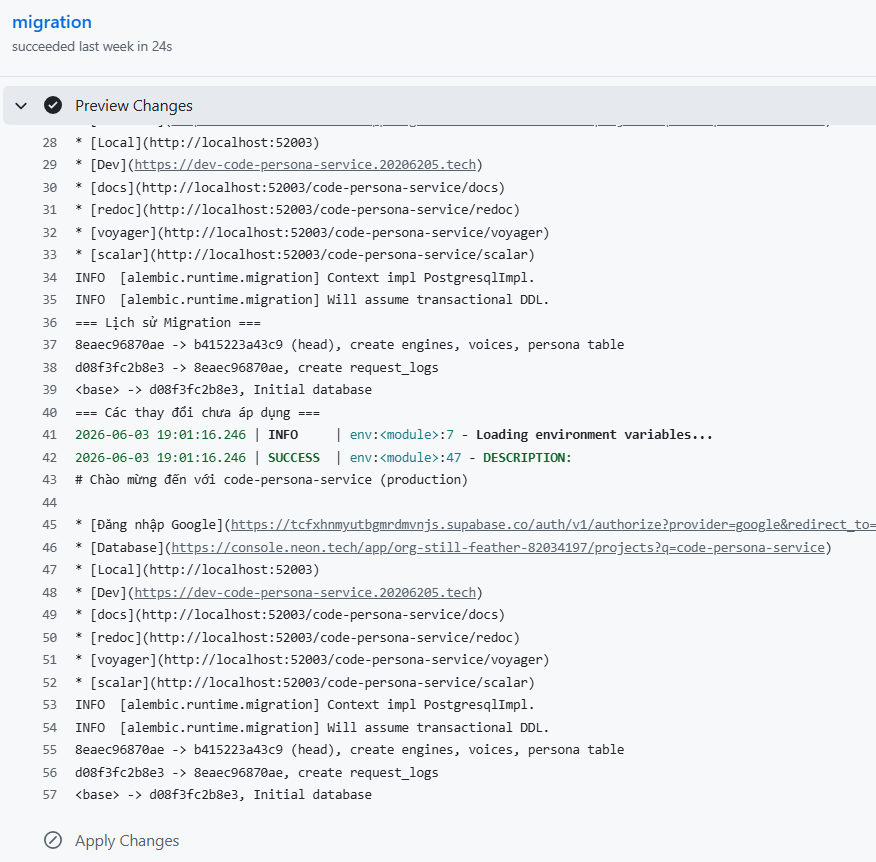
\includegraphics[width=0.8\textwidth]{pictures/persona-database-migration.png}
\caption{Quản lý di chuyển CSDL của dịch vụ nhân vật}
\end{figure}

Cấu trúc các bảng trong CSDL của dịch vụ nhân vật:

\begin{figure}[H]
\centering
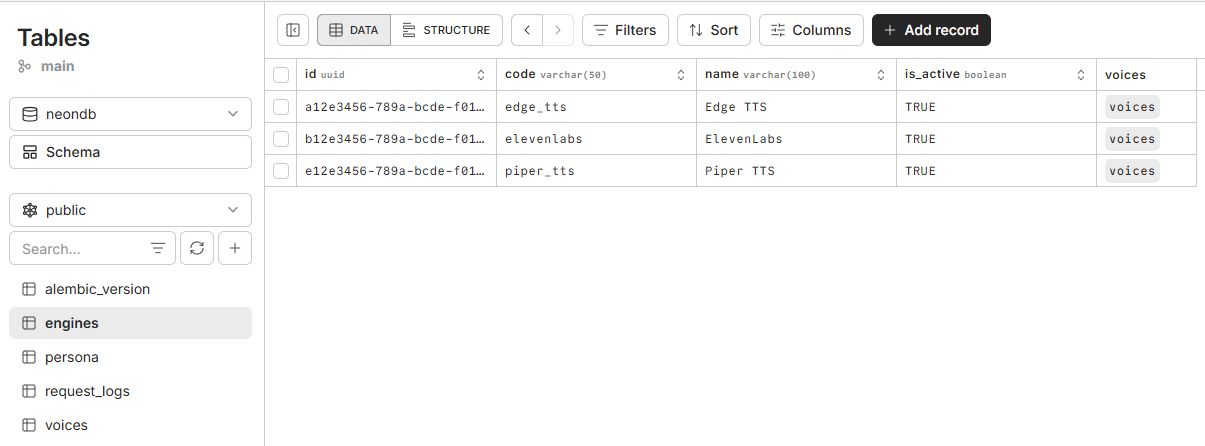
\includegraphics[width=0.8\textwidth]{pictures/persona-database.png}
\caption{Cấu trúc các bảng trong CSDL của dịch vụ nhân vật}
\end{figure}

%%%%%%%%%%%%%%%%%%%%%%%%%%%%%%%%%%%%%%
% Mô tả chi tiết thông tin bảng trong CSDL
%%%%%%%%%%%%%%%%%%%%%%%%%%%%%%%%%%%%%%
% thứ tự các bảng trong tài liệu

\begin{table}[H]
\centering
\begin{tabular}{|l|l|p{6cm}|}
\hline
\textbf{Cột} & \textbf{Kiểu dữ liệu} & \textbf{Mô tả} \\ \hline
version\_num & varchar & Mã phiên bản di chuyển CSDL hiện tại của Alembic. \\ \hline
\end{tabular}
\caption{Cấu trúc bảng \texttt{alembic\_version} (Dịch vụ nhân vật)}
\end{table}

\begin{table}[H]
\centering
\begin{tabular}{|l|l|p{6cm}|}
\hline
\textbf{Cột} & \textbf{Kiểu dữ liệu} & \textbf{Mô tả} \\ \hline
id & uuid & Khóa chính của log yêu cầu HTTP. \\ \hline
request\_id & varchar & \\ \hline
method & varchar & Phương thức HTTP được sử dụng. \\ \hline
url & varchar & \\ \hline
client\_ip & varchar & \\ \hline
status\_code & int4 & Mã trạng thái phản hồi HTTP trả về. \\ \hline
request\_payload & json & \\ \hline
response\_payload & json & \\ \hline
process\_time & float8 & \\ \hline
created\_at & timestamptz & Thời gian ghi nhận log hệ thống. \\ \hline
\end{tabular}
\caption{Cấu trúc bảng \texttt{request\_logs} (Dịch vụ nhân vật)}
\end{table}

\begin{table}[H]
\centering
\begin{tabular}{|l|l|p{6cm}|}
\hline
\textbf{Cột} & \textbf{Kiểu dữ liệu} & \textbf{Mô tả} \\ \hline
id & uuid & Khóa chính của công cụ/mô hình AI. \\ \hline
code & varchar & \\ \hline
name & varchar & Tên của engine/model tương ứng. \\ \hline
is\_active & bool & \\ \hline
\end{tabular}
\caption{Cấu trúc bảng \texttt{engines} (Dịch vụ nhân vật)}
\end{table}

\begin{table}[H]
\centering
\begin{tabular}{|l|l|p{6cm}|}
\hline
\textbf{Cột} & \textbf{Kiểu dữ liệu} & \textbf{Mô tả} \\ \hline
voice\_uuid & uuid & \\ \hline
voice\_code & varchar & \\ \hline
engine\_id & uuid & ID engine liên kết tương ứng. \\ \hline
is\_active & bool & \\ \hline
\end{tabular}
\caption{Cấu trúc bảng \texttt{voices} (Dịch vụ nhân vật)}
\end{table}

\begin{table}[H]
\centering
\begin{tabular}{|l|l|p{6cm}|}
\hline
\textbf{Cột} & \textbf{Kiểu dữ liệu} & \textbf{Mô tả} \\ \hline
id & uuid & Khóa chính định danh nhân vật ảo. \\ \hline
name & varchar & Tên của nhân vật ảo. \\ \hline
gender & varchar & \\ \hline
voice\_uuid & uuid & \\ \hline
description & text & \\ \hline
avatar\_url & varchar & Đường dẫn URL ảnh đại diện của nhân vật ảo. \\ \hline
greeting\_audio\_url & varchar & Đường dẫn URL file âm thanh chào hỏi của nhân vật. \\ \hline
greeting\_text & text & Đoạn trò chuyện chào hỏi mặc định của nhân vật dạng văn bản. \\ \hline
is\_active & bool & \\ \hline
created\_at & timestamp & Thời gian tạo nhân vật. \\ \hline
updated\_at & timestamp & Thời gian cập nhật cấu hình nhân vật. \\ \hline
\end{tabular}
\caption{Cấu trúc bảng \texttt{persona} (Dịch vụ nhân vật)}
\end{table}
